\documentclass[12pt]{IEEEtran}

\usepackage{algorithm, algpseudocode, amsmath, cite, graphicx, icomma, multirow, url, xspace}

%\hyphenation{}
\newcommand{\latex}{\LaTeX\xspace}
\renewcommand\thesection{\arabic{section}}
\renewcommand\thesubsection{\thesection.\arabic{subsection}}
\renewcommand\thesubsubsection{\thesubsection.\arabic{subsubsection}}

\renewcommand\thesectiondis{\arabic{section}}
\renewcommand\thesubsectiondis{\thesectiondis.\arabic{subsection}}
\renewcommand\thesubsubsectiondis{\thesubsectiondis.\arabic{subsubsection}}

\begin{document}

\title{Document Conversion to \latex\ with OCR}
\author{Logan~Short, Christopher~Wong, and~David~Zeng}% <-This % stops a space
\markboth{CS 231A Final Project, Winter 2015}{}
\maketitle

\begin{abstract}
agg
\end{abstract}

\section{Introduction}

\IEEEPARstart{O}{ptical} character recognition (OCR) is the process of converting images of typed or handwritten text into digital characters. In particular, we are considering the problem of using OCR techniques to turn an image of a typesetted document into \latex, a markup language commonly used to typeset scientific literature. The motivation for our problem comes from the fact that many old books and academic papers exist online only as scanned images, and to be able to convert these images into formattable \latex documents would allow these documents to be much more easily maintained by websites and readers. These documents could also be indexed and searched by search engines, and perhaps in the future we will be able to query academic papers directly with \latex markup.

\section{Related Work in OCR}

agg

\subsection{Summary of Previous Work}

In \cite{1}, Jacobs et al.

In \cite{2}, Frey and Slate

In \cite{3}, Gupta et al. discuss methods for identifying document layout structure from images of documents. The key intuition behind the algorithm proposed in \cite{3} is that the various components of documents, in this case technical papers, can be identified using the features of the bounding boxes encapsulating each section as well as the realtive positioning and ordering of said bounding boxes. Gupta et al. first preprocess their document images by thresholding at 80\% of the image intensity. Characters in the document are then located by identifying contours in the thresholded image and bounding boxes are formed around these characters. Bounding boxes that are close together are then combined horizontally to yield line level bounding boxes and combined vertically to obtain paragraph level bounding boxes. Following the construction of the paragraph level bounding boxes, features such as aspect ratio and average line height are used to differentiate between textual components and graphical components. At this point the the known strucutre of technical papers is leveraged to classify the previously found bounding boxes as various document components. An image representation is generated in which the previously found bounding boxes are indicated by filled white rectangles while the rest of the image is black. Horizontal and vertical image profile histograms of this image are then used to classify bounding boxes as containing the document title, authors, abstract, main body, and other layout components using known qualities of technical papers. For example, the title is a textual component located at the top of the document, has a high aspect ratio and is immediately followed by the authors filed. Once the bounding boxes are all classified as layout components of the document, the document is classified as one of several common technical paper formats, e.g. IEEE or LNCS. The format determined through classification then cements the layout structure of the document.

In \cite{4}, Tapia and Rojas describes an algorithm for learning the appropriate \latex layout for a handwritten mathematical expression. The paper assumes that for a given expression, the individual symbols in the expressions have already been discovered and labeled, and a bounding box has been drawn around each. Given such a setup, Tapia and Rojas define a concept they call dominance. Each symbol dominates a region around it; for example, a summation symbol dominates the region above and below it, where subexpressions are usually located that define the range for the summation. To construct the appropriate \latex layout for the expression, Tapia and Rojas notice that \latex markup essentially forms a tree structure, where arguments, subscripts, and superscripts are essentially children of some given parent symbol. They devise a method for learning this tree structure. Each symbol is treated as a node and edges between two symbols are weighted based on the distance between the centroids of the bounding boxes of the two symbols. First, the concept of dominance is used to find a dominant baseline of symbols in an expression. The remaining symbols are attached to this baseline by finding the minimum spanning tree that includes the baseline. In terms of the \latex structure, the dominant baseline provides the sequence of top level symbols, whereas the branches of the minimum spanning tree that connect to the baseline are the arguments, superscripts, and subscripts of the baseline symbols. If these branches off of the baseline are complex enough, this process is recursively applied to find baselines for each branch, from which smaller minimum spanning trees are then built of the baseline for each of the branches.

\subsection{Main Contributions of Our Work}
TODO Expand on this. How are we using previous work in our project? 2-3 sentences.
The goal of our project is to create an end-to-end system that takes in as input an image of a typesetted document and outputs the matching \latex for the document. Our main contribution resides not so much in improving upon the OCR techniques described in the previous work, but rather in designing a top-down approach for converting a document image into \latex by building upon smaller modules that utilize the OCR techniques in previous literature. Many of the OCR techniques we have cited are targeted at isolated problems such as recognition of handwritten characters or math equations. Since we are instead concerned with full images of typesetted documents, the technical challenges at each level of our system are related to but slightly different from those discussed in the corresponding prior works. Details of the techniques we use in our implementation will be discussed in Section 3.2.

\section{Implementation}

We begin by giving an overview of our system in Section 3.1, and in Section 3.2, we give specific implementation details of each part of our algorithm.

\subsection{Summary of Implementation}
The key tasks in constructing a \latex representation from an image of a document are extracting the document contents and information from the image and converting this information into \latex form.

OCR techniques for extracting information from a document achieve the highest accuracy when the document is oriented in a left to right and top to bottom manner. Scans or photos of documents are not always of optimal quality and thus document images are not guaranteed to be oriented exactly in this ideal fashion. It is therefore advantageous for our algorithm to first rotate the document image to the proper orientation before any other techniques for extracting document information are utilized.

Given a document image whose orientation is properly aligned in a left to right and top to bottom manner, the next step in extracting document contents is to identify the sections of the image that contain textual information. Focusing on these sections exclusively allows for finer tuned character recognition and information extraction. In general, for academic papers document information is primarily contained in plain text sections and display mode equation blocks. The next phase of our implementation thus deciphers which parts of the document image correspond to these information containing sections. The structure of information differs between the two types of information blocks, thus during this step it is important to record the type of a document section as well as its location in the image.

Analyzing blocks of text is performed using a hierarchical approach. The algorithm begins by splitting text blocks into lines of text. Each of these lines of text is then split into its component words and the text of each word is then determined using a text classifier. The deciphered word texts are then concatenated horizontally to form textual representations of each line and these lines are then concatenated vertically to obtain the contents of the text block.

Identifying the contents of display mode equation sections uses a similar approach where the section is broken down  into its individual equations. Each equation is then analyzed to obtain a \latex representation. The \latex layout for each equation is learned using the method in \cite{4} described in section 2.1. The obtained \latex representations are then encapsulated into a display mode \latex block which is returned as the contents of the equation section.

After the contents of each document section are extracted from the image, a \latex representation of the document is constructed by concatenating the contents of each individual section in the top to bottom order in which they appear. Layout is kept simple as the main focus of the implementation is to maximize the accuracy of the data contained in the document.

\subsection{Implementation Details}

agg

\subsubsection{Rotation Fixing}

agg

\subsubsection{Text and Equation Sectioning}

agg

\subsubsection{Text Analyzing}

agg

\subsubsection{Equation Analyzing}

%% TEMPLATE FOR ADDING IMAGES. SPANS ONE COLUMN.
% \begin{figure}[h]
%   \centering
%     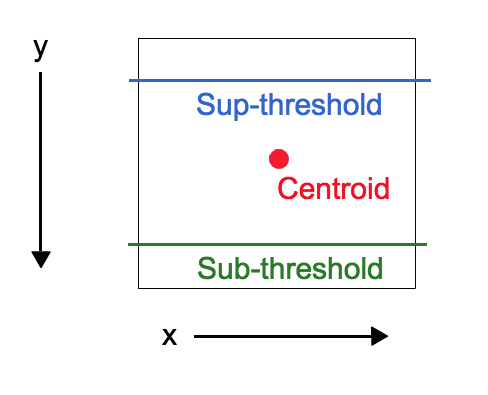
\includegraphics[width=3.2in]{values.png}
%   \caption{An example image.}
%   \label{fig:values}
% \end{figure}
% Look at me. I'm citing Figure~\ref{fig:values}.
%% TEMPLATE FOR ADDING IMAGES. SPANS ONE COLUMN.

Transforming images of single line mathematical expressions requires us to not only recognize individual symbols used in the expression, but also the layout of the expression. To perform this, we used a simplified version of the method used in \cite{4}, which we will now describe in detail.

TODO: describe how to get from symbols to bounding boxes.

Each bounding box of a symbol is described by four values, the $(x,y)$ coordinates of the top-left corner of the box and the width and height of the box. Coordinates of pixels in the image have $x$ values that increase from left to right and $y$ values that increase from top down.
For each bounding box detected in the image for an expression, we define the following terms. The \textit{centroid} of a symbol is a point in the bounding box that indicates, roughly, where the center of the symbol lies. The \textit{sup-threshold} of a symbol denotes the upper bound for the $y$ value of a superscript, while the \textit{sub-threshold} denotes the lower bound for the $y$ value of a subscript. Figure \ref{fig:values} gives a visual representation for each of these definitions. Each symbol is categorized as one of three types: \textit{ascendant}, \textit{descendant}, \textit{central}. These distinctions allow us to distinguish characters where

\begin{figure}[h]
  \centering
    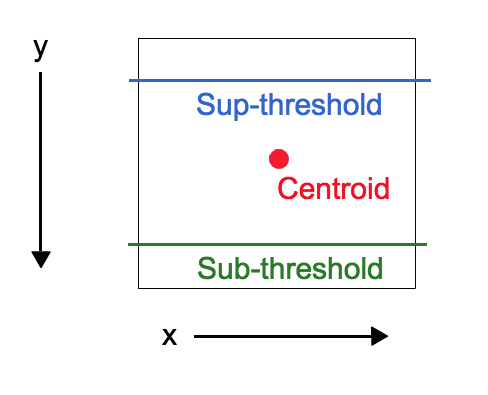
\includegraphics[width=3.2in]{values.png}
  \caption{points and lines of interest for a bounding box}
  \label{fig:values}
\end{figure}

One of the main ideas presented in \cite{4} is the concept of dominance. Each symbol is capable of dominating some subset of five different regions: \textit{above}, \textit{below}, \textit{superscript}, \textit{subscript}, and \textit{subexpression}. The locations of each of these regions, relative to the bounding box, is show in Figure \ref{fig:locations}.

\begin{figure}[h]
  \centering
    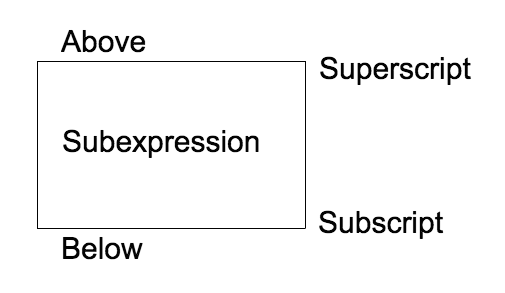
\includegraphics[width=3.2in]{locations.png}
  \caption{dominated regions of a symbol}
  \label{fig:locations}
\end{figure}

Symbols in expressions fall into three categories: ascendant, descendant, and centered.




\subsubsection{Latex Construction}

agg

\section{Experimentation Results}

agg

\section{Conclusion}

agg

\begin{thebibliography}{1}
\bibitem{1} C. Jacobs, P. Simard, P. Viola, J. Rinker. Text Recognition of Low-resolution Document Images. Microsoft, 2005.
\bibitem{2} P. Frey, D. Slate. Letter Recognition Using Holland-Style
Adaptive Classifiers. Machine Learning, 1991. \\
\bibitem{3} G. Gupta, S. Niranjan, A. Shrivastava. Document Layout Analysis \& Classification and Its Application in OCR. EDOCW, 2006. \\
\bibitem{4} E. Tapia, R. Rojas. Recognition of On-line Handwritten Mathematical Expressions Using a Minimum Spanning Tree Construction and Symbol Dominance. LNCS, 2004.
\end{thebibliography}

%\balancecolumns

\end{document}
